\section{Auswertung}
\label{sec:Auswertung}
Alle in der Auswertung benutzten Mittelwerte werden über die Gleichung
\begin{equation}
\tilde{x}=\frac{1}{n}\sum_{i=1}^n {x_i}
\end{equation}
bestimmt. Die Standardabweichung der Mittelwerte ergibt sich zu 
\begin{equation}
\Delta{\tilde{x}}=\sqrt{\frac{1}{n(n-1)}\sum_{i=1}^n {(x_i-\tilde{x})²}}.
\end{equation}
Wird eine Größe bestimmt, welche sich aus fehlerbehafteten Daten zusammensetzt, ergibt sich der absolute Fehler über die Gaussche Fehlerfortpflanzung 
\begin{equation}
\Delta{f}(x_1,..,x_n)=\sqrt{\left(\frac{\mathup{d}f}{\mathup{d}x_1}\Delta{x_1}\right)²+..+\left(\frac{\mathup{d}f}{\mathup{d}x_n}\Delta{x_n}\right)²}.
\end{equation}
Zur Berechnung aller Größen werden die nicht gerundeten Größen benutzt um Rundungsfehler zu vermeiden. Am Ende der Auswertung aller Größen werden diese auf die erste signifikante Stelle des Fehlers gerundet. 

\subsection{Gamma-Strahlung}
Der Nulleffekt für beide Messungen ergibt sich durch den Quotienten der gemessenen Zerfälle $n$ pro Zeiteinheit ${\mathup{\Delta{t}}}$ zu
\begin{equation}
N_\mathup{u}=\frac{n}{\mathup{\Delta{t}}}=\frac{682}{\SI{750}{\second}}=0,91\,\frac{1}{\si\second}.
\end{equation}
Es werden der Absorptionskoeffizient $\mu$ und $N_0$ für Blei und Eisen bestimmt. Dabei werden die Materialien der Strahlung eines $\ce{^{137}Cs}$--Strahlers ausgesetzt. 
\subsubsection{Blei-Strahlung}

\begin{table}
\centering
\begin{tabular}{S[table-format=2.1] S[table-format=3.0] S[table-format=5.0] S[table-format=3.2] S[table-format=1.2]}
\toprule
{$d\:/\si{\milli\meter}$} & {$t\:/\si\second$} & {$n$} & {$N-N_\mathup{u}$} & {$\ln{(N-N_\mathup{u})}$}\\
\midrule
 1.2 &   80 & 10700 &  132.84 & 4.89\\
 1.3 &   80 & 10630 &  131.97 & 4.88\\
 2.4 &   80 &  8919 &   48.31 & 3.88\\
 6.0 &   80 &  6690 &   17.89 & 2.88\\
10.3 &  120 &  5906 &    5.89 & 1.77\\
12.9 &  120 &  4569 &  110.58 & 4.71\\
20.2 &  180 &  3383 &   14.42 & 2.67\\
21.4 &  120 &  1840 &   82.72 & 4.42\\
30.5 &  180 &  1223 &    1.96 & 0.67\\
40.4 &  180 &  516  &   37.17 & 3.62\\
\bottomrule
\end{tabular}
\caption{Gemessene und berechnete Werte der Strahlungsintensität zu für verschiedene Schichtdicken und Messzeiten für Blei.}
\label{tab:werte_gamma_blei}
\end{table}
In \ref{tab:werte_gamma_blei} sind die Messwerte, sowie die um denn Nulleffekt $N_\mathup{u}$ korrigierten Intensitäten aufgetragen. der Logarithmus der korrigierten Intensität wird im weiteren Verlauf benötigt und ist ebenfalls dargestellt. Zwischen der Schichtdicke $d$ und dem Logarithmus der Intensität ergibt sich ein linearer Zusammenhang. 
\begin{figure}
	\centering
	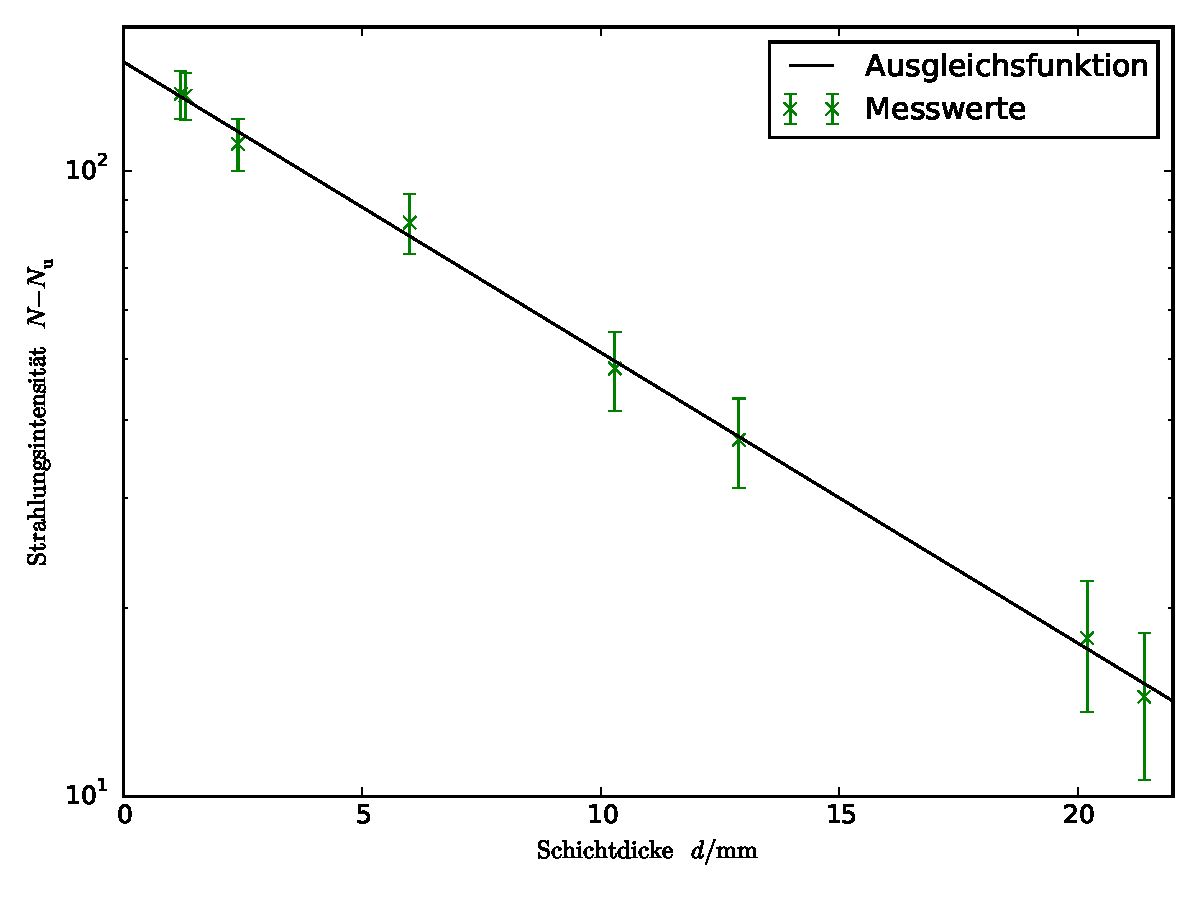
\includegraphics[width=0.9\textwidth]{Bilder/Blei.pdf}
	\caption{Schichtdicke $d$ aufgetragen gegen die Strahlungsintensität.}
	\label{fig:blei}
\end{figure}
Durch lineare Regression wird dieser in Abbildung \ref{fig:blei} aufgezeigt. Aus der Geradengleichung
\begin{equation}
f(x)=(-107,0\pm0,9)x+(5,01\pm0,02)
\end{equation}
ergebens sich für den Absorptionskoeffizient $\mu=-(107,0\pm0,9)\,\frac{1}{\si\meter}$ und den Anfangswert $N_0=(150\pm1)\,\frac{1}{\si\second}$.

%Damit ist das Absorptionsgesetz nach THeorie
%\begin{equation}
%N(d)=(150\pm1)\,\frac{1}{\si\second}\cdot\exp{[-(107,0\pm0,9)\,\frac{1}%{\si\meter}d]}
%\end{equation}
%ist.
\subsubsection{Eisen-Strahlung}
\begin{table}
\centering
\begin{tabular}{S[table-format=2.1] S[table-format=3.0] S[table-format=5.0] S[table-format=3.2] S[table-format=1.2]}
\toprule
{$d\:/\si{\milli\meter}$} & {$t\:/\si\second$} & {$n$} & {$N-N_\mathup{u}$} & {$\ln{(N-N_\mathup{u})}$}\\
\midrule
 0.5 &   80 & 11878 & 147.57 & 4.99\\
 1.5 &   80 & 11284 & 140.14&  4.94\\
 3.0 &   80 & 10345 & 128.40 & 4.86\\
 5.0 &   80 &  9563 & 118.63 & 4.78\\
 5.0 &  120 &  8007 &  65.82 & 4.19\\
10.0 &  120 & 11095 &  91.55 & 4.52\\
20.0 &  120 &  6402 &  52.44 & 3.96\\
25.0 &  180 &  7622 &  41.44 & 3.72\\
30.0 &  180 &  5958 &  32.19 & 3.47\\
40.0 &  180 &  3254  & 17.17 & 2.84\\
\bottomrule
\end{tabular}
\caption{Gemessene und berechnete Werte der Strahlungsintensität zu für verschiedene Schichtdicken und Messzeiten für Eisen.}
\label{tab:werte_gamma_eisen}
\end{table}
In \ref{tab:werte_gamma_eisen} sind die Messwerte, sowie die um denn Nulleffekt $N_\mathup{u}$ korrigierten Intensitäten aufgetragen. der Logarithmus der korrigierten Intensität wird im weiteren Verlauf benötigt und ist ebenfalls dargestellt. Zwischen der Schichtdicke $d$ und dem Logarithmus der Intensität ergibt sich ein linearer Zusammenhang. 
\begin{figure}
	\centering
	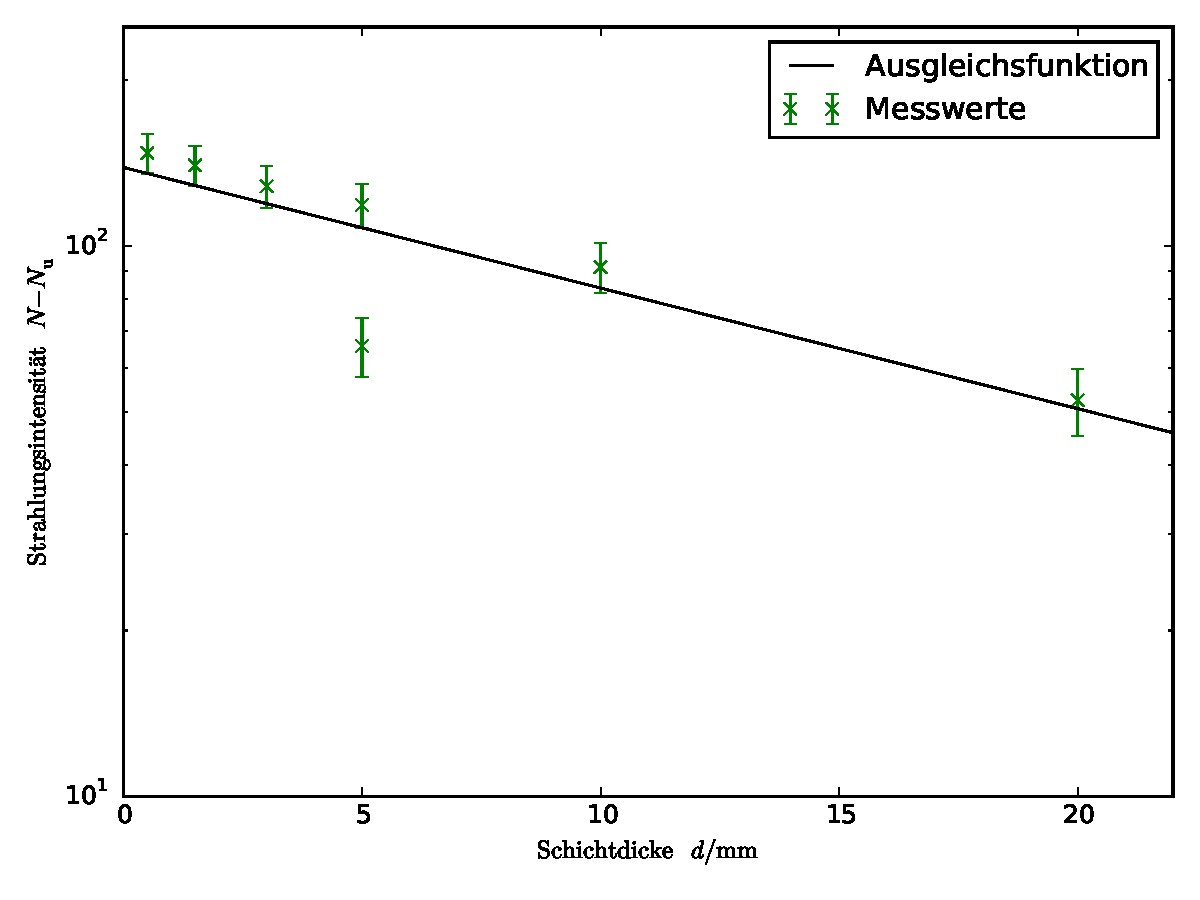
\includegraphics[width=0.9\textwidth]{Bilder/Eisen.pdf}
	\caption{Schichtdicke $d$ aufgetragen gegen die Strahlungsintensität.}
	\label{fig:eisen}
\end{figure}
Durch lineare Regression wird dieser in Abbildung \ref{fig:eisen} aufgezeigt. Aus der Geradengleichung
\begin{equation}
f(x)=(-50\pm5)x+(4,93\pm0,09)
\end{equation}
ergebens sich für den Absorptionskoeffizient $\mu=-(50\pm5)\,\frac{1}{\si\meter}$ und den Anfangswert $N_0=(138\pm1)\,\frac{1}{\si\second}$.
\subsection{Maximale Energie der Strahlung}


Erneut wird der Nulleffekt $N_\mathup{u}$ zu 
\begin{equation}
N_\mathup{u}=\frac{\text{Zerfälle}}{\text{Zeit}}=\frac{273}{\SI{750}{\second}}=0.364\,\frac{1}{\si\second}
\end{equation}
bestimmt. 

\begin{table}
\centering
\begin{tabular}{S[table-format=3.1(2)] S[table-format=3.0] S[table-format=5.0] S[table-format=2.3]}
\toprule
{$d\:/\si{\micro\meter}$} & {$t\:/\si\second$} & {$n$} & {$I$}\\
\midrule
102(1)   & 350 &18401 & 52.210\\
126(1)   & 350 & 8934 & 25.516\\
153.0(5) & 350 & 3693 & 10.187\\
160(1)   & 350 & 2230 &  6.007\\
200(1)   & 350 &  736 &  1.739\\
253(1)   & 350 &  225 &  0.279\\
302(1)   & 500 &  199 &  0.034\\
338(5)   & 500 &  187 &  0.010\\
400(1)   & 500 &  211 &  0.058\\
444(2)   & 500 &  271 &  0.178\\
\bottomrule
\end{tabular}
\caption{Korrigierte und zur Rechnung benötigte Winkel der Spektrallinien.}
\label{tab:werte_beta}
\end{table}


Die Intensität $I$ ergibt sich aus der Differenz $I=N-N_\mathup{u}$ und ist mit der Schichtdicke $d$, der Messzeit $t$ und der Anzahl der Zerfälle $n$ in Tabelle \ref{tab:werte_beta} gelistet.


 Wird die Intensität halblogarithmisch gegen die Schichtdicke aufgetragen kann die maximale Reichweite der $\beta$-Teilchen durch den Schnitt zweier Geraden ermittelt werden. Diese entstehen durch lineare Regression der Werte X und Y. Die zweite Gerade hat die Steigung m=0.
Der Schnitt kann berechnet werden über 
\begin{equation}
R_\mathup{max}=\frac{b_2-b_1}{m_2-m_1}.
\end{equation}
Nach Theorie kann daraus die maximale Energie bestimmt werden. Dies ist jedoch sehr ungenau oder sonst irgendwie doof, deswegen geschieht das nun über den empirischen Zusammenhang aus Theorie.
\begin{figure}
	\centering
	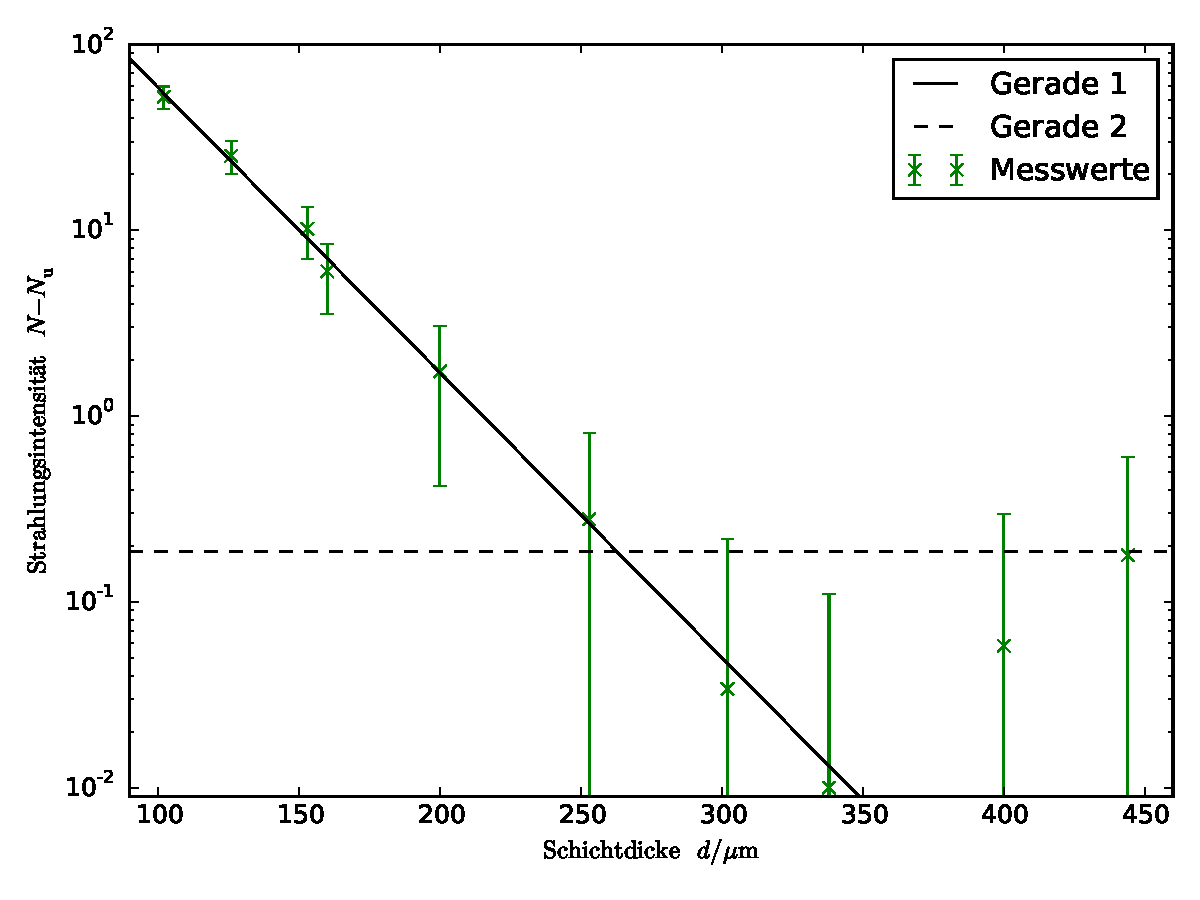
\includegraphics[width=0.9\textwidth]{Bilder/beta.pdf}
	\caption{Reichweite des Schallimpulses in Abhängigkeit von der Laufzeit, Regression zur Bestimmung der Geschwindigkeit.}
	\label{fig:geschwindigkeit}
\end{figure}


